\def\year{2021}\relax
%File: formatting-instructions-latex-2021.tex
%release 2021.1
\documentclass[letterpaper]{article} % DO NOT CHANGE THIS
\usepackage{aaai21}  % DO NOT CHANGE THIS
\usepackage{times}  % DO NOT CHANGE THIS
\usepackage{helvet} % DO NOT CHANGE THIS
\usepackage{courier}  % DO NOT CHANGE THIS
\usepackage[hyphens]{url}  % DO NOT CHANGE THIS
\usepackage{graphicx} % DO NOT CHANGE THIS

% ADJUSTED BY AFM ----------------------------------------------------------
\usepackage{amsmath} % ENTERED BY AFM

\urlstyle{rm} % DO NOT CHANGE THIS
\def\UrlFont{\rm}  % DO NOT CHANGE THIS
\usepackage{natbib}  % DO NOT CHANGE THIS AND DO NOT ADD ANY OPTIONS TO IT
\usepackage{caption} % DO NOT CHANGE THIS AND DO NOT ADD ANY OPTIONS TO IT
\frenchspacing  % DO NOT CHANGE THIS
\setlength{\pdfpagewidth}{8.5in}  % DO NOT CHANGE THIS
\setlength{\pdfpageheight}{11in}  % DO NOT CHANGE THIS
\nocopyright
%PDF Info Is REQUIRED.
% For /Author, add all authors within the parentheses, separated by commas. No accents or commands.
% For /Title, add Title in Mixed Case. No accents or commands. Retain the parentheses.
\pdfinfo{
/Title (ML Assignment 1)
/Author (Anthony Menninger)
/TemplateVersion (2021.1)
} %Leave this
% /Title ()
% Put your actual complete title (no codes, scripts, shortcuts, or LaTeX commands) within the parentheses in mixed case
% Leave the space between \Title and the beginning parenthesis alone
% /Author ()
% Put your actual complete list of authors (no codes, scripts, shortcuts, or LaTeX commands) within the parentheses in mixed case.
% Each author should be only by a comma. If the name contains accents, remove them. If there are any LaTeX commands,
% remove them.

% DISALLOWED PACKAGES
% \usepackage{authblk} -- This package is specifically forbidden
% \usepackage{balance} -- This package is specifically forbidden
% \usepackage{color (if used in text)
% \usepackage{CJK} -- This package is specifically forbidden
% \usepackage{float} -- This package is specifically forbidden
% \usepackage{flushend} -- This package is specifically forbidden
% \usepackage{fontenc} -- This package is specifically forbidden
% \usepackage{fullpage} -- This package is specifically forbidden
% \usepackage{geometry} -- This package is specifically forbidden
% \usepackage{grffile} -- This package is specifically forbidden
% \usepackage{hyperref} -- This package is specifically forbidden
% \usepackage{navigator} -- This package is specifically forbidden
% (or any other package that embeds links such as navigator or hyperref)
% \indentfirst} -- This package is specifically forbidden
% \layout} -- This package is specifically forbidden
% \multicol} -- This package is specifically forbidden
% \nameref} -- This package is specifically forbidden
% \usepackage{savetrees} -- This package is specifically forbidden
% \usepackage{setspace} -- This package is specifically forbidden
% \usepackage{stfloats} -- This package is specifically forbidden
% \usepackage{tabu} -- This package is specifically forbidden
% \usepackage{titlesec} -- This package is specifically forbidden
% \usepackage{tocbibind} -- This package is specifically forbidden
% \usepackage{ulem} -- This package is specifically forbidden
% \usepackage{wrapfig} -- This package is specifically forbidden
% DISALLOWED COMMANDS
% \nocopyright -- Your paper will not be published if you use this command
% \addtolength -- This command may not be used
% \balance -- This command may not be used
% \baselinestretch -- Your paper will not be published if you use this command
% \clearpage -- No page breaks of any kind may be used for the final version of your paper
% \columnsep -- This command may not be used
% \newpage -- No page breaks of any kind may be used for the final version of your paper
% \pagebreak -- No page breaks of any kind may be used for the final version of your paperr
% \pagestyle -- This command may not be used
% \tiny -- This is not an acceptable font size.
% \vspace{- -- No negative value may be used in proximity of a caption, figure, table, section, subsection, subsubsection, or reference
% \vskip{- -- No negative value may be used to alter spacing above or below a caption, figure, table, section, subsection, subsubsection, or reference

\setcounter{secnumdepth}{0} %May be changed to 1 or 2 if section numbers are desired.

% The file aaai21.sty is the style file for AAAI Press
% proceedings, working notes, and technical reports.
%

% Title

% Your title must be in mixed case, not sentence case.
% That means all verbs (including short verbs like be, is, using,and go),
% nouns, adverbs, adjectives should be capitalized, including both words in hyphenated terms, while
% articles, conjunctions, and prepositions are lower case unless they
% directly follow a colon or long dash


%Example, Single Author, ->> remove \iffalse,\fi and place them surrounding AAAI title to use it
\title{
Machine Learning - CS 7641
Assignment 3
	
}
\author {
    % Author
    Anthony Menninger \\
}

\affiliations{
    Georgia Tech OMSCS Program \\
    amenninger3\\
    tmenninger@gatech.edu

}

\begin{document}

\maketitle

\begin{abstract}
This paper explores several unsupervised learning algorithms.  It uses two datasets: Census Data labeled to income above or below \$50,000 and MNIST handwritten digit image data for digits 0-9.  Clustering is performed on the original datasets, then several dimensionality techniques are used to reduced the feature set and then clustering is preformed again.  Finally, the reduced datasets are tested using learning algorithms.  
\end{abstract}

\section{Introduction}
The first data set is from 1994 and 1995 current population surveys conducted by the U.S. Census Bureau [2] from the UC Irvine Machine learning site.  The classification task is to determine if the user type for each instance has an income above \$50,000 or below (\$94,000 in today's dollars).  There are 40 usable features, with both continuous features, such as age, and discrete, such as married status or sex.  The training set has 199,523 instances and the test set has 99,762 instances.  Because many of the features in the file are string based, I created transformed instances using the sklearn preprocessing LabelEncoder to translate discrete string values into consistent numeric values.  This was necessary for algorithms that only used numeric features. I chose this data set because it the training dataset seemed relatively large and I expect somewhat noisy with a smallish number of features.  

The second data set is The MNIST Database of Handwritten Digits [2].  This consists of instances of 28 X 28 greyscale images of the digits 0-9.  One transformation performed was that the values where scaled to 0 to 1, from 0 to 255.  The images were flattened, creating 784 features, one for each pixel.  There are 60,000 training instances and 10,000 test instances.  I chose this because it is a good comparison to the first data set, with a very different type of data (images), which leads to significantly more features (784).  In addition, each of the features can be thought of as related to each other, as they are all positional in a two dimensional grid, while the first data set features do not have any necessary relation between themselves ie:  age is not related to sex.   

For this assignment, the core python library used was sklearn [3], which has many unsupervised learning algorithms.  In addition, an enhancement Yellowbrick [4] was also used for some visualizations.


\section{Clustering}
\subsection{K Means}
K Means creates K clusters based on the distance of instances to cluster centers.  A key question is what is the optimal number of clusters.  An Elbow Plot looks at the intra distance within clusters at different K, and then picks the K where intra-distance change slows down, or the "elbow" of the plot.  A silhouette plot charts the  intra cluster distance and references it vs the next nearest cluster intra cluster distance.  This produces a chart that can provide visual insight.  Both methods were used in choosing an optimal K.

\begin{figure}[!htb]
\centering
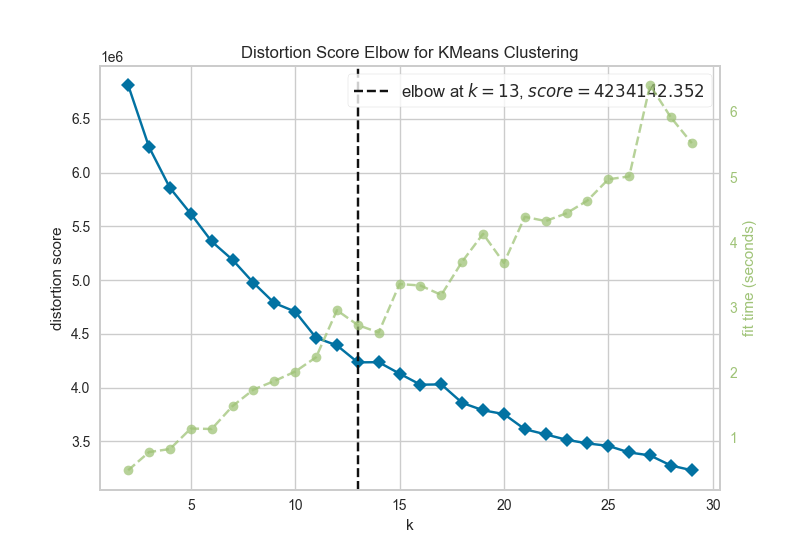
\includegraphics[width=2.75in, height=2.75in]{figures/Census_elbow_max_30_best_13.png}
\caption{K Means Census Elbow:  . }
\label{fig:kmeans_census_elbow}
\end{figure}

\textbf{Figure \ref{fig:kmeans_census_elbow}} shows the elbow chart score


\begin{figure}[!htb]
\centering
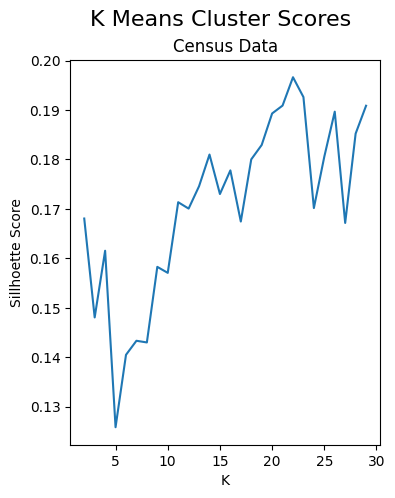
\includegraphics[width=2.75in, height=2.75in]{figures/K_Means_Cluster_Scores_Census_Data.png}
\caption{K Means Census Data Silhouette Scores:  . }
\label{fig:kmeans_census_silhouette}
\end{figure}

 \textbf{Figure \ref{fig:kmeans_census_silhouette}} shows the silhoette score
 
 \begin{figure}[!htb]
\centering
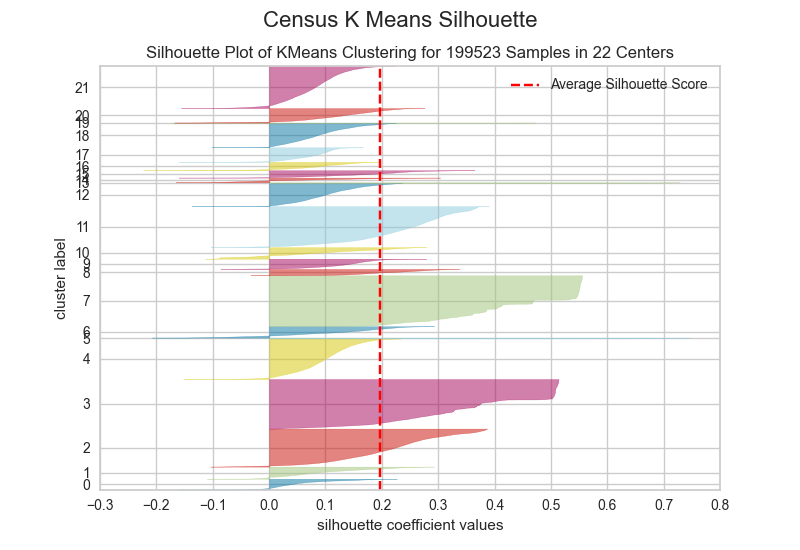
\includegraphics[width=2.75in, height=2.75in]{figures/Census_silhouette_K_22.png}
\caption{K Means Census Best Silhouette:  . }
\label{fig:kmeans_census_silhouette_best}
\end{figure}

 \textbf{Figure \ref{fig:kmeans_census_silhouette}} shows the silhoette score
  \textbf{Figure \ref{fig:kmeans_census_silhouette_best}} shows the silhoette score


\section{References}
\begin{tabular}{l p{2.75in}}
\\
1 & The MNIST Database of Handwritten Digits. url: http://yann.lecun.com/exdb/mnist/.
\\
2 & Census Income (KDD). url: https://archive-beta.ics.uci.edu/ml/datasets/census+income+kdd.
\\
3 & Scikit-learn: Machine Learning in Python, Pedregosa et al., JMLR 12, pp. 2825-2830, 2011.
\\
4 & Bengfort et al., (2019). Yellowbrick: Visualizing the Scikit-Learn Model Selection Process. Journal of Open Source Software, 4(35), 1075, https://doi.org/10.21105/joss.01075.
\\
4 & Menninger, A. (2022)  Code created for this experiment https://github.com/BigTMiami/ML\_Assign\_2  Created: 2022.
\end{tabular}
\end{document}
